\documentclass[journal]{IEEEtran}

\usepackage{cite}
% http://www.ctan.org/tex-archive/macros/latex/contrib/cite/
\usepackage[pdftex]{graphicx}
\graphicspath{{./img/}}
\DeclareGraphicsExtensions{.pdf,.jpeg,.png}
\usepackage{algorithmicx}
% http://www.ctan.org/tex-archive/macros/latex/contrib/algorithmicx/
\usepackage{array}
% http://www.ctan.org/tex-archive/macros/latex/required/tools/
\usepackage{mdwtab}
% http://www.ctan.org/tex-archive/macros/latex/contrib/mdwtools/
\usepackage{eqparbox}
% http://www.ctan.org/tex-archive/macros/latex/contrib/eqparbox/
\usepackage[caption=false,font=footnotesize]{subfig}
% http://www.ctan.org/tex-archive/macros/latex/contrib/subfig/
\usepackage{fixltx2e}
% http://www.ctan.org/tex-archive/macros/latex/base/
\usepackage{stfloats}
% http://www.ctan.org/tex-archive/macros/latex/contrib/sttools/
\usepackage{url}
% http://www.ctan.org/tex-archive/macros/latex/contrib/misc/

% correct bad hyphenation here
\hyphenation{op-tical net-works semi-conduc-tor}


\begin{document}

\title{WWW-Graphics-Module for Mixed-Reality-System}

\author{Hannes~Eilers,~\textit{Master-student,~Chairman~student~group~NorthernStars,~FH-Kiel,}
        Eike~Petersen,~\textit{Master-student,~FH-Kiel}}

% The paper headers
\markboth{Advanced JavaScript project paper, January~2014}%
{Shell \MakeLowercase{\textit{et al.}}: WWW-Graphics-Module for Mixed-Reality-System}

\maketitle

\begin{abstract}
	Warum? Was? Wie? (Max 200 W)
\end{abstract}
\begin{IEEEkeywords}
mixed-reality, javascript, server, client, paper.
\end{IEEEkeywords}

\section{Introduction}

\IEEEPARstart{T}{he}
Mixed-Reality is a robocup soccer league that uses hardware and software
simulation to develop artificial intelligences (AIs) for robots. The system
used for playing in competitions all over the world uses a horizontal screen, that
simulates a soccer field with field lines, goals and a ball. On the screen are
real robots with quadratic dimensions for each side of nearly 25cm. A game
server uses a vision system above the screen for tracking the robots and
generating a worldmodel that includes positions of all robots as well as
simulated objects like goals or important flags on the field. By using a
infrared transmitter the server can send commands to the robots.\\
For each robot a seperate process can connect to the game server to control the
speed of the right and left wheel or the robot. The gameserver sends the
worldmodel to this process, so that it can react to changes on the field.\\
The Mixed-Reality system uses several modules to track and control the robots or
to display the field on the screen.\\
During a competition one AI for each robot connects to the game server using a
local network and team leaders next tof the soccer field can request timeouts to
change the behaviour of a AI or replace the robots for kick offs.

\subsection{Project definition (Was machen wir?)}
The projects goal is to bring the local mixed-reality-games to an audience everywhere in the world (Figure~\ref{fig:proj_goal}). All that is needed is a device with a HTML-5 compliant Browser and an internet-connection with a bit-rate of at least 10-kbit/s downstream.
The primarily targeted devices are pcs, tablets and smart-phones but not limited to those. \\
The games should be streamed in real-time from the mixed-reality game-server over a web-server to in-browser RICH-clients, where they will be displayed in the same fashion as the local mixed-reality-game graphics.
\begin{figure}[!t]
    \centering
    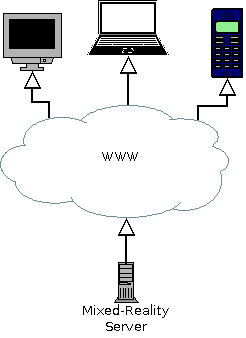
\includegraphics[width=0.3\textwidth]{project-target.png}
    \caption{Project goal: Bringing MR to you!}
    \label{fig:proj_goal}
\end{figure}
\subsection{Design (Wie sieht es aus?)}
As in Figure~\ref{fig:proj_design} shown, the web-server is capable to establish a connection to any Mixed-Reality game-server and game over UDP. This connection is interchangeable an internal game representation, that converts the incoming XML to JSON and verifies it, manages the listening clients and encapsulates needed administrative functions. The verified JSON is sent over websockets at a fixed interval to the clients, (Canvas und so? RICH-Client usw)
\begin{figure}[!t]
    \centering
    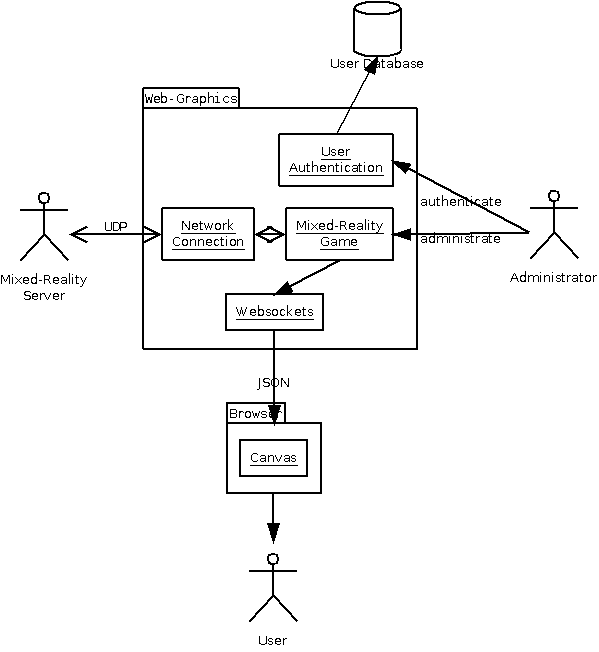
\includegraphics[width=0.3\textwidth]{design.png}
    \caption{Project design}
    \label{fig:proj_design}
\end{figure}
\subsection{Implementation(Wie ist es aufgebaut?)}
\subsubsection{Server}
The design for the server is implemented as a proof-of-concept on the server-framework Node.js~\cite{Node.js} with most of the needed configuration and essentials implemented with the middle-ware express~\cite{express}, such as session-management, URL-routing and serving of static files. The Website is constructed through templates with the template-engine jade~\cite{jade} and also served through express.\\
The user-persistence is handled by an sqlite-database with sqlite3~\cite{sqlite3}, because of its convenience to setup and redesign in a agile software development environment~\cite{agile_devel} and the ease of conversion to a better setup when the project reaches maturity.\\
The communication besides http is managed by websocket.io~\cite{websocket.io}\cite{smash_node.js}, an extension to express.\\ 
To decode the incoming XML xml2js~\cite{xml2js} is used and to build an easy to manage and debug system extensive logging is done with log4js~\cite{log4js} an conversion of the Java logging package log4j2~\cite{log4j2}.\\
Design Pattern, special things\\[3mm]
\subsubsection{Client}
\section{Conclusion}
Ergebnis Auswertung und weitere Aussichten

\section*{Acknowledgment}

The authors would like to thank...

\begin{thebibliography}{1}

\bibitem{Node.js}
Joyent,~Inc, \emph{Node.js}, \url{http://nodejs.org/}.
\bibitem{express}
expressjs.com, \emph{express web~application~framework~for~node}, \url{http://expressjs.com/}.
\bibitem{jade}
jade-lang.com, \emph{jade Node~Template~Engine}, \url{http://jade-lang.com/}.
\bibitem{sqlite3}
MapBox, \emph{node-sqlite3 - Asynchronous, non-blocking SQLite3 bindings for Node.js}, \url{https://github.com/mapbox/node-sqlite3}.
\bibitem{agile_devel}
K.~Beck, \emph{Extreme~programming~eXplained : embrace~change}, 2nd~ed. Addison-Wesley, 2005.
\bibitem{websocket.io}
G.~Rauch, \emph{websocket.io}, \url{https://npmjs.org/package/websocket.io}.
\bibitem{smash_node.js}
G.~Rauch, \emph{SMASHING~Node.js JavaScript~Everywhere}, 1st~ed. WILEY, 2012.
\bibitem{xml2js}
Leonidas-from-XIV, \emph{node-xml2js}, \url{https://github.com/Leonidas-from-XIV/node-xml2js}.
\bibitem{log4js}
nomiddlename, \emph{log4js-node}, \url{https://github.com/nomiddlename/log4js-node}.
\bibitem{log4j2}
Apache Software Foundation, \emph{Apache Log4j 2}, \url{http://logging.apache.org/log4j/2.x/index.html}.

\end{thebibliography}

\end{document}


